\chapter{Results}
Table \ref{tab:Optical2} shows the fractions estimated from the analysis of the BPT diagnostic diagrams for the two samples collecting galaxies selected as BCG and non-BCG, according to the selection on signal-to-noise ratio (SNR) greater than 3 and aligning non-BCGs to the same redshift range as BCGs. This filtering resulted in a set of 149 and 78 galaxies, respectively, for the BPT-[NII] and BPT-[SII] diagrams in the BCG sample. In the same context, there were 98,571 and 88,867 galaxies for the non-BCG sample.
To evaluate AGN activity, particularly in the BPT-[SII] diagnostic diagram, the combination of the Seyfert and LINER categories allows a further estimation of the maximum percentage. Analyzing the results presented in Table \ref{tab:Optical2} , the fraction of AGN in the BCGs sample range from 58$\%$ to 74$\%$. In the corresponding context, non-BCGs exhibit percentages in the range of 12$\%$ to 13$\%$. These values are consistent with the findings of \cite{2012A&A...546A..17V}, even if the results they report are derived from a larger sample that includes BCGs and sources with a SNR also lower than 3.
This calculations indeed show that BCGs show a greater optical AGN fraction, than non BCGs.
A further analysis was also implemented by dividing the BCG sample into four bins with the same number of elements and calculating the AGN fractions for both samples in relation to these bins.
Results of the latter, depicted in Fig.\ref{IMG:frac_z}, suggest that although the AGN fraction for non-BCGs shows a slight increase within the redshift range of BCGs (i.e., $0.02 \leq z \leq 0.1$), the corresponding percentages for BCGs remain constant at a value of 65/70$\%$, as depicted in Fig.\ref{IMG:frac_z}. Such an increase could not be detected with these calculations in the BCG sample, due to both smaller statistics and a broader dispersion of errors, but these results cannot exclude it. In this context, for future developments, it would be interesting to analyze the reasons behind the broader dispersion of errors for the fraction of non-BCGs at lower redshift.

Lastly, the analysis dedicated for detecting the BCGs and non-BCGs associated with radio loud emission indicates that BCGs are more likely to host radio luminosity exceeding 5mJy at 1.4 GHz, with a fraction of $12\%$. This value is 20 times higher than the fraction found for the non-BCG subsample of galaxies within the selected regions, as discussed earlier, corresponding to $0.6\%$.

%COSE TENUTE PER SICUREZZA MA MIGLIORATE E DUNQUE DEPRECATE !
\begin{comment}

 The additional selection in redshift significantly altered the information captured by the census of both samples. Specifically, within BCGs in Table \ref{tab:Optical}, the vast majority of species are at least suspected to host an AGN, rather than exhibiting prevalent star-forming characteristics. However, when looking at the same values in Table \ref{tab:Optical2}, the suspicion becomes almost a certainty.
Meanwhile, the BPT-[SII] analysis goes further, defining the main feedback coming from such AGNs. It is evident in Tables \ref{tab:Optical} and \ref{tab:Optical2} that the main population of AGNs shows low ionization ratios.
This change, resulting from the further selection in redshift, also alters the information obtained from non-BCGs census. Initially, the BPT-[SII] findings indicate that most objects detected as Composite appear to be star-forming galaxies. However, with the subsequent selection in redshift, this assumption becomes less certain, leading to a better subdivision between Liners and SF galaxies.

In \ref{tab:Optical}, detailing the results of the optical analysis, it is observed that BCGs are more likely to host an AGN compared to ordinary galaxies. Percentages obtained for the non-BCG sample are consistent with Vitale et al. \cite{2012A&A...546A..17V}. 

It is noteworthy that the percentages obtained for the non-BCG sample align with the findings of Vitale et al. \cite{2012A&A...546A..17V}. This observation leads to the conclusion that BCGs are more likely to exhibit AGN activity, as discussed in the previous context of percentages.

\begin{table}[htb]
  \centering
  \begin{tabular}{cccc}
    \hline\hline
    \multicolumn{1}{c}{Diagram} & Classification & non-BCG & BCG \\
    \hline
    [NII]  & AGNs &  $52896 \pm 84$ ($21.1 \pm 0.03$)$\%$ &$161 \pm 5$ ($50.4 \pm 1.6$)$\%$ \\
           & Composites & $55875 \pm 110$ ($22.3 \pm 0.04$)$\%$ & $110 \pm 5$ ($34.5 \pm 1.8$)$\%$ \\
           & SFGs & $141753 \pm 80$ ($56.6 \pm 0.03$)$\%$ &$ 49 \pm 4$ ($15.4 \pm 1.4$)$\%$ \\ 
    \hline
    [SII]  & Seyferts & $13082 \pm 64$ ($6.3 \pm 0.03$)$\%$  &$8 \pm 2$ ($6.5 \pm 1.6$)$\%$\\
           & LINERs & $28396 \pm 80$ ($13.6 \pm 0.04$)$\%$ & $74 \pm 3$ ($53.3 \pm 2.4$)$\%$ \\
           & SFGs &$167826\pm 76 $ ($80.2 \pm 0.04$)$\%$ & $55 \pm 3$ ($40.2 \pm 2.2$)$\%$\\ 
    \hline\hline
  \end{tabular}
  \caption{Results of the classification using BPT diagnostic diagrams, according to the criteria established by Kewley et al. \cite{2006MNRAS.372..961K}. The outcomes are presented in terms of counts per region and as a percentage for each population. }
  \label{tab:Optical}
\end{table}

\end{comment}
%Da riportare nel testo !!!!!!!!
%PER BCG NII ci sono 149
%PER BCG SII ci sono 78
%PER NON NII ci sono 98'571
%PER NON SII 88'867
\begin{table}[htb]
  \centering
  \begin{tabular}{cccc}
    \hline\hline
    \multicolumn{1}{c}{Diagram} & Classification & non-BCG & BCG \\
    \hline
    [NII]  & AGNs & $12.04 \pm 0.03$ $\%$ & $58.0 \pm 1.8$ $\%$ \\
           & Composites & $17.49 \pm 0.05$ $\%$ &  $34.7 \pm 2.2$ $\%$ \\
           & SFGs & $70.47 \pm 0.03$ $\%$ &  $7.3 \pm 0.2$ $\%$ \\ 
    \hline
    [SII]  & Seyferts & $4.22 \pm 0.03$ $\%$  & $6.6 \pm 1.7$ $\%$\\
           & LINERs & $9.03 \pm 0.04$ $\%$  & $67.6 \pm 2.5$ $\%$\\
           & SFGs &$86.75 \pm 0.04$ $\%$  & $25.9 \pm 2.1$ $\%$\\
    \hline\hline
  \end{tabular}
  \caption{Results of the classification using BPT diagnostic diagrams, following the criteria established by Kewley et al. \cite{2006MNRAS.372..961K}. The samples were additionally refined by requiring a signal-to-noise ratio (SNR) greater than 3 and aligning non-BCGs within the same redshift range as BCGs. The results are presented as percentages for each population. }
  \label{tab:Optical2}
\end{table}

\begin{figure}[t]
  \centering
  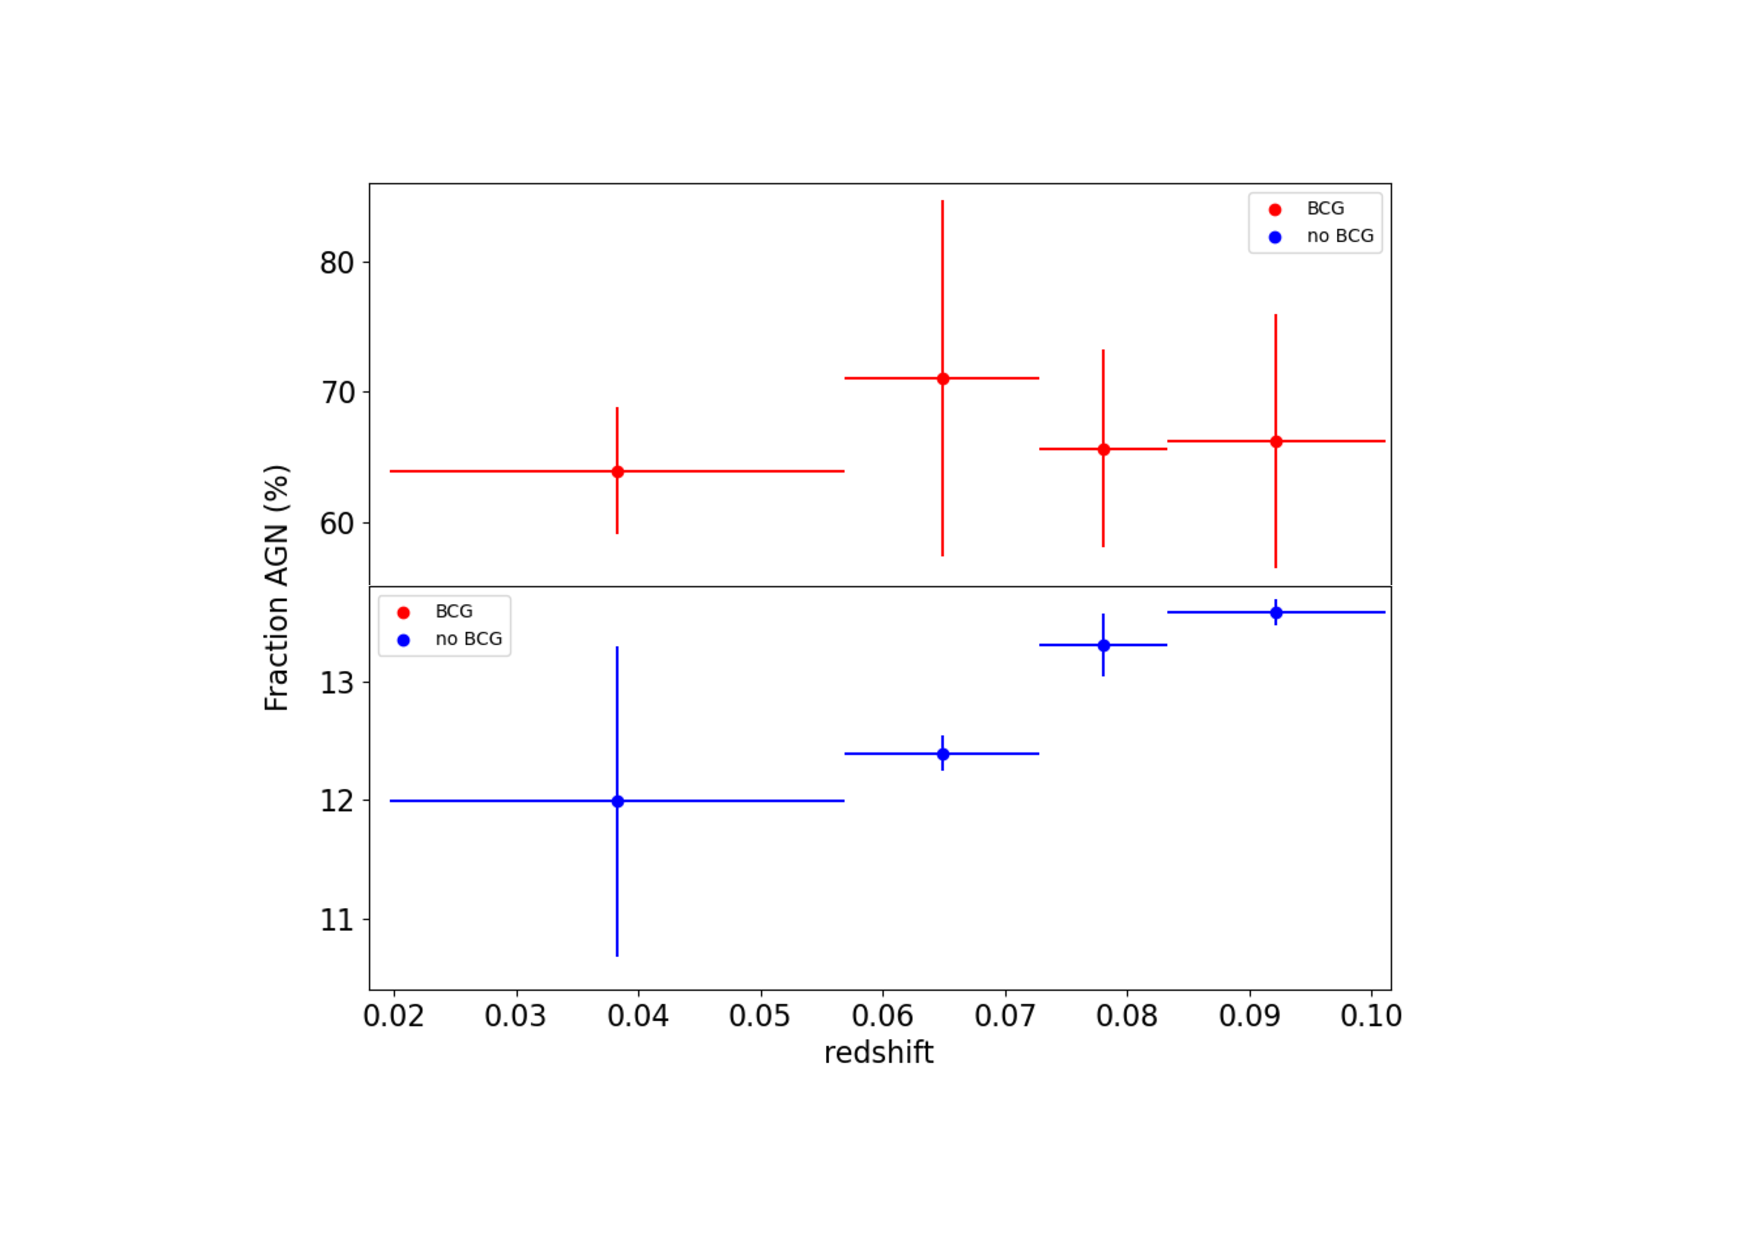
\includegraphics[width=0.85\textwidth]{zfractionAGN}
  \caption{Visual representation illustrating the absence of redshift fluctuation in AGN activity percentages, specifically as AGN in the BPT [NII] diagnostic diagram and as Seyfert + LINER in the BPT [SII] diagnostic diagram. Redshift bins are uniformly defined to maintain consistent BCG statistics within each bin. The samples underwent further refinement by imposing a signal-to-noise ratio (SNR) threshold greater than 3, and aligning non-BCGs within the identical redshift range as BCGs.}
  \label{IMG:frac_z}
\end{figure}

